\documentclass[12pt,a4paper]{article}

\usepackage[utf8]{inputenc}
\usepackage[T5]{fontenc}
\usepackage[vietnamese]{babel}
\usepackage{lmodern}
\usepackage[a4paper,left=25mm,right=20mm,top=22mm,bottom=22mm]{geometry}
\usepackage{amsmath}
\usepackage{booktabs}
\usepackage{longtable}
\usepackage{array}
\usepackage{xcolor}
\usepackage{listings}
\usepackage{enumitem}
\usepackage{caption}
\usepackage{graphicx}
\usepackage{float}
\usepackage{tikz}
\usepackage[hidelinks]{hyperref}

\usetikzlibrary{arrows.meta,positioning}

\definecolor{codebg}{RGB}{245,247,249}
\definecolor{codegreen}{RGB}{20,110,60}
\definecolor{flowblue}{RGB}{38,94,145}

\lstset{
  basicstyle=\ttfamily\small,
  backgroundcolor=\color{codebg},
  frame=single,
  breaklines=true,
  columns=fullflexible,
  keepspaces=true,
  showstringspaces=false,
  commentstyle=\color{codegreen},
  keywordstyle=\color{blue!70!black}
}

\newcommand{\code}[1]{\texttt{\detokenize{#1}}}
\newcommand{\um}{$\,\mu\mathrm{m}$}
\newcommand{\umsq}{$\,\mu\mathrm{m}^{2}$}
\graphicspath{{../Pictures/}}

\newcommand{\reportfigure}[3][0.88\textwidth]{%
  \begin{figure}[H]
    \centering
    \includegraphics[width=#1,height=0.72\textheight,keepaspectratio]{#2}
    \caption{#3}
  \end{figure}
}

\newcommand{\reportpair}[5]{%
  \begin{figure}[H]
    \centering
    \begin{minipage}[t]{0.48\textwidth}
      \centering
      \includegraphics[width=\linewidth,height=0.35\textheight,keepaspectratio]{#1}
      \caption*{(a) #2}
    \end{minipage}\hfill
    \begin{minipage}[t]{0.48\textwidth}
      \centering
      \includegraphics[width=\linewidth,height=0.35\textheight,keepaspectratio]{#3}
      \caption*{(b) #4}
    \end{minipage}
    \caption{#5}
  \end{figure}
}

\title{\textbf{Thiết kế CPU 4-bit bằng quy trình thiết kế vi mạch số trên OpenLane 2}}
\author{Võ Minh Huy -- MSSV: 22207042\\
Nguyễn Trần Huy Tưởng -- MSSV: 23207125}
\date{\today}

\begin{document}

\maketitle

\begin{abstract}
Báo cáo trình bày quá trình thiết kế một CPU 4-bit từ mô tả RTL
SystemVerilog đến layout GDSII trên công nghệ SkyWater 130\,nm. Quy trình
bao gồm xây dựng kiến trúc, mô phỏng RTL, tổng hợp logic, floorplan,
placement, clock-tree synthesis, routing, trích xuất ký sinh, mô phỏng
post-layout và xuất GDSII. Thiết kế đạt timing với clock 20\,ns, antenna
0 violation, có kết nối nguồn đầy đủ và tạo được artifact GDSII. Signoff
đạt 0 DRC violation trên KLayout và LVS match uniquely.
\end{abstract}

\tableofcontents
\newpage

\section{Giới thiệu}

Mục tiêu của đề tài là minh họa đầy đủ quy trình thiết kế ASIC số thông
qua một CPU có datapath 4-bit. Thiết kế đủ nhỏ để dễ quan sát nhưng vẫn
chứa các thành phần quan trọng như ALU, thanh ghi, program counter, bộ
điều khiển FSM, clock, reset và giao tiếp bộ nhớ chương trình.

Luồng thiết kế được thực hiện theo trình tự:

\begin{center}
\begin{tikzpicture}[
  node distance=4mm,
  box/.style={
    draw=flowblue,
    rounded corners,
    fill=blue!5,
    minimum height=8mm,
    minimum width=30mm,
    align=center,
    font=\small
  },
  arrow/.style={-{Latex[length=2mm]},thick,draw=flowblue}
]
\node[box] (rtl) {Thiết kế RTL};
\node[box,right=of rtl] (sim) {Mô phỏng RTL};
\node[box,right=of sim] (syn) {Synthesis};
\node[box,below=of syn] (fp) {Floorplan};
\node[box,left=of fp] (place) {Placement};
\node[box,left=of place] (cts) {CTS};
\node[box,below=of cts] (route) {Routing};
\node[box,right=of route] (rcx) {Parasitic\\extraction};
\node[box,right=of rcx] (gls) {Post-layout\\STA/GLS};
\node[box,below=of gls] (gds) {GDSII};
\node[box,left=of gds] (signoff) {DRC/LVS};

\draw[arrow] (rtl) -- (sim);
\draw[arrow] (sim) -- (syn);
\draw[arrow] (syn) -- (fp);
\draw[arrow] (fp) -- (place);
\draw[arrow] (place) -- (cts);
\draw[arrow] (cts) -- (route);
\draw[arrow] (route) -- (rcx);
\draw[arrow] (rcx) -- (gls);
\draw[arrow] (gls) -- (gds);
\draw[arrow] (gds) -- (signoff);
\end{tikzpicture}
\end{center}

\section{Công nghệ và công cụ}

\begin{longtable}{>{\raggedright\arraybackslash}p{0.27\textwidth}
                  >{\raggedright\arraybackslash}p{0.63\textwidth}}
\toprule
\textbf{Thành phần} & \textbf{Vai trò} \\
\midrule
\endhead
SystemVerilog & Mô tả RTL của CPU, ALU, control unit và testbench. \\
Xcelium & Mô phỏng RTL và gate-level simulation có SDF. \\
Yosys & Tổng hợp RTL và ánh xạ sang standard cell. \\
OpenROAD & Floorplan, placement, CTS, routing, STA và trích xuất ký sinh. \\
OpenLane 2 & Cung cấp môi trường, PDK và các bước kiểm tra signoff. \\
Sky130A & PDK SkyWater 130\,nm sử dụng trong thiết kế. \\
\code{sky130_fd_sc_hd} & Thư viện standard cell high-density. \\
Magic, KLayout và Netgen & DRC, stream-out, extraction và LVS. \\
\bottomrule
\end{longtable}

Clock mục tiêu có chu kỳ 20\,ns, tương đương 50\,MHz. Floorplan sử dụng
core utilization mục tiêu 65\%.

\section{Thiết kế RTL}

\subsection{Kiến trúc CPU}

CPU sử dụng datapath 4-bit và instruction 8-bit. Mỗi instruction gồm
opcode 4-bit và operand 4-bit. Operand được sử dụng làm dữ liệu immediate
hoặc địa chỉ nhảy.

Ba khối RTL chính gồm:

\begin{itemize}[noitemsep]
  \item \code{cpu_4bit}: top-level chứa program counter, instruction
        register, accumulator và các cờ trạng thái;
  \item \code{control_unit}: giải mã instruction và điều khiển FSM gồm
        FETCH, EXECUTE và HALT;
  \item \code{alu_4bit}: thực hiện các phép số học, logic và dịch bit.
\end{itemize}

Instruction memory được đặt bên ngoài core. CPU chỉ xuất địa chỉ
\code{imem_addr[3:0]} và nhận instruction qua
\code{imem_rdata[7:0]}. Cách tổ chức này giúp physical design chỉ chứa
logic CPU và không tổng hợp ROM mô phỏng thành standard cell.

\subsection{Tập lệnh}

\begin{longtable}{>{\centering\arraybackslash}p{0.12\textwidth}
                  >{\raggedright\arraybackslash}p{0.15\textwidth}
                  >{\raggedright\arraybackslash}p{0.56\textwidth}}
\toprule
\textbf{Opcode} & \textbf{Lệnh} & \textbf{Chức năng} \\
\midrule
\endhead
\code{0x0} & NOP & Không thay đổi trạng thái CPU. \\
\code{0x1} & LDI & Nạp operand vào ACC. \\
\code{0x2} & ADD & Cộng operand với ACC. \\
\code{0x3} & SUB & Trừ operand khỏi ACC. \\
\code{0x4} & AND & AND giữa ACC và operand. \\
\code{0x5} & OR  & OR giữa ACC và operand. \\
\code{0x6} & XOR & XOR giữa ACC và operand. \\
\code{0x7} & NOT & Đảo các bit của ACC. \\
\code{0x8} & SHL & Dịch trái ACC một bit. \\
\code{0x9} & SHR & Dịch phải logic ACC một bit. \\
\code{0xA} & JMP & Nhảy không điều kiện đến operand. \\
\code{0xB} & JZ  & Nhảy đến operand nếu cờ zero bằng 1. \\
\code{0xC} & INC & Tăng ACC lên 1. \\
\code{0xD} & DEC & Giảm ACC đi 1. \\
\code{0xF} & HLT & Dừng CPU. \\
\bottomrule
\end{longtable}

\subsection{ALU 4-bit}

ALU hỗ trợ bốn nhóm thao tác:

\begin{itemize}[noitemsep]
  \item số học: cộng, trừ, tăng và giảm;
  \item logic: AND, OR, XOR và NOT;
  \item dịch bit: dịch trái và dịch phải logic;
  \item truyền operand trực tiếp để thực hiện LDI.
\end{itemize}

Các cờ zero, carry, borrow, negative và overflow được cập nhật sau những
lệnh ghi kết quả vào ACC.

\section{Mô phỏng và kiểm chứng RTL}

Testbench tạo clock 20\,ns và mô hình instruction memory bất đồng bộ,
zero-wait-state. Chương trình kiểm thử gồm:

\begin{center}
\code{LDI 3} $\rightarrow$
\code{ADD 5} $\rightarrow$
\code{SUB 2} $\rightarrow$
\code{SHL} $\rightarrow$
\code{SHR} $\rightarrow$
\code{HLT}.
\end{center}

Giá trị ACC thay đổi lần lượt thành 3, 8, 6, 12 và 6. Sau lệnh HLT,
\code{halted} lên mức 1. Testbench tự kiểm tra và trả về:

\begin{lstlisting}
TEST PASSED: ACC = 6
\end{lstlisting}

\reportfigure[0.66\textwidth]{1.png}
{Kết quả mô phỏng RTL: ACC thay đổi đúng theo chuỗi lệnh, CPU vào trạng
thái HALT và testbench báo \code{TEST PASSED: ACC = 6}.}

Kết quả này xác nhận chức năng cơ bản của RTL trước khi chuyển sang
synthesis và physical design.

\reportfigure{2.png}
{Mô phỏng RTL đầy đủ đến 250\,ns: địa chỉ tăng từ 0 đến 6, instruction lần lượt là
\code{13}, \code{25}, \code{32}, \code{80}, \code{90}, \code{F0} và
\code{00}; tín hiệu \code{halted} lên mức 1 sau lệnh HLT.}

\section{Tổng hợp logic}

Yosys đọc ba file RTL tổng hợp được, tối ưu logic và ánh xạ thiết kế sang
thư viện \code{sky130_fd_sc_hd}. Testbench và program ROM không được đưa
vào synthesis.

\begin{longtable}{>{\raggedright\arraybackslash}p{0.48\textwidth}
                  >{\raggedleft\arraybackslash}p{0.32\textwidth}}
\toprule
\textbf{Chỉ tiêu} & \textbf{Kết quả} \\
\midrule
\endhead
Top module & \code{cpu_4bit} \\
Số wire sau technology mapping & 140 \\
Số standard-cell instance & 140 \\
Số flip-flop \code{dfrtp_2} sau tối ưu & 19 \\
Mapped cell area & 1591.5264\umsq \\
\bottomrule
\end{longtable}

\reportfigure[0.72\textwidth]{3.png}
{Kết quả tổng hợp của Yosys sau technology mapping: thiết kế gồm 140
standard cell với tổng diện tích 1591.5264\umsq.}

Netlist sau tổng hợp là đầu vào của OpenROAD.
Trước khi link design, flow đọc technology LEF, standard-cell LEF và
Liberty ở corner TT, 25\,$^\circ$C, 1.80\,V
(\code{sky130_fd_sc_hd__tt_025C_1v80}). Sau đó netlist được link với top
\code{cpu_4bit} và file
\code{manual_constraints.sdc} được nạp để khởi tạo STA đúng.

\begin{lstlisting}[language=tcl]
read_lef $TECH_LEF
read_lef $CELL_LEF
read_liberty sky130_fd_sc_hd__tt_025C_1v80.lib
read_verilog cpu_4bit.nl.v
link_design cpu_4bit
read_sdc manual_constraints.sdc
\end{lstlisting}

Constraint tạo clock 20\,ns (50\,MHz), clock uncertainty 0.25\,ns và
input/output delay 4\,ns. Các output có tải pin 0.0334; clock, reset và
bus dữ liệu vào được mô hình hóa bởi driving cell
\code{sky130_fd_sc_hd__inv_2}. Flow cũng giới hạn transition 0.75,
capacitance 0.20 và fanout tối đa 10. Initial STA cho setup worst slack
$+14.71$\,ns, hold worst slack $+0.27$\,ns và TNS bằng 0.

Utilization được báo là 100\% trước floorplan chỉ là giá trị tạm: ở thời
điểm đó chưa có placement area để làm mẫu số. Giá trị này không phải mật
độ thực của implementation.

\reportfigure[0.62\textwidth]{4.png}
{Initial STA sau khi nạp netlist và constraint: setup slack
$+14.71$\,ns, hold slack $+0.27$\,ns và TNS bằng 0.}

\section{Floorplan và power planning}

\subsection{Cấu hình chính}

\begin{longtable}{>{\raggedright\arraybackslash}p{0.35\textwidth}
                  >{\raggedright\arraybackslash}p{0.50\textwidth}}
\toprule
\textbf{Tham số} & \textbf{Giá trị} \\
\midrule
\endhead
PDK & \code{sky130A} \\
Standard-cell library & \code{sky130_fd_sc_hd} \\
Clock port & \code{clk} \\
Clock period & 20\,ns \\
Target core utilization & 65\% \\
Aspect ratio & 1.0 \\
\bottomrule
\end{longtable}

Target utilization 65\% tạo sự cân bằng giữa diện tích core và khoảng
trống cần thiết cho placement, clock buffer, timing repair và routing.
Đây là giá trị dùng để tính kích thước floorplan ban đầu; utilization
cuối có thể thay đổi sau khi flow chèn thêm cell.

\begin{lstlisting}[language=tcl]
initialize_floorplan -utilization 65 \
  -aspect_ratio 1.0 \
  -core_space {10.88 10.88 5.52 5.52} \
  -site unithd
make_tracks
\end{lstlisting}

\reportfigure[0.82\textwidth]{5.png}
{Floorplan sau khi tạo die, core và placement rows, tiếp theo là các
routing track được tạo bởi \code{make_tracks}.}

\reportpair{6a.png}
{Báo cáo trước floorplan: chưa có placement area nên utilization tạm là
100\%}
{6b.png}
{Báo cáo sau floorplan: tạo 18 placement row, utilization 66\% và timing
vẫn đạt}
{Đối chiếu báo cáo thiết kế trước và sau khi khởi tạo floorplan.}

\subsection{Bố trí I/O}

Các chân được nhóm theo chức năng:

\begin{itemize}[noitemsep]
  \item \code{imem_addr[3:0]} ở cạnh Bắc;
  \item \code{imem_rdata[7:0]} ở cạnh Nam;
  \item \code{clk} và \code{rst_n} ở cạnh Tây;
  \item \code{halted} ở cạnh Đông.
\end{itemize}

Cách bố trí này giữ các bus liên quan ở cùng một cạnh và giúp routing dễ
quan sát. Tapcell và endcap được chèn để nối well/substrate đúng cách và
bảo vệ biên của các hàng standard cell.

\begin{lstlisting}[language=tcl]
place_pins -hor_layers met3 -ver_layers met2 \
  -corner_avoidance 5 -min_distance_in_tracks
tapcell -distance 13 \
  -tapcell_master sky130_fd_sc_hd__tapvpwrvgnd_1 \
  -endcap_master sky130_fd_sc_hd__decap_3
\end{lstlisting}

\reportpair{7a.png}
{Bố trí các chân I/O}
{7b.png}
{Kết quả lệnh pin placement}
{Bố trí và kiểm tra các chân I/O.}

\subsection{Power Planning}

Power distribution network sử dụng hai net \code{VPWR} và \code{VGND}.
Các rail trên met1 cấp nguồn trực tiếp cho hàng standard cell; stripe trên
met4 và met5 phân phối nguồn trong core. Sau khi tạo PDN, connectivity của
hai net nguồn được kiểm tra trước khi placement và routing.

\begin{lstlisting}[language=tcl]
global_connect
set_voltage_domain -name CORE -power VPWR -ground VGND
define_pdn_grid -name stdcell_grid \
  -voltage_domain CORE -pins {met4 met5}
pdngen
check_power_grid -net VPWR
check_power_grid -net VGND
\end{lstlisting}

\reportfigure[0.82\textwidth]{8.png}
{Power Distribution Network (PDN) sau \code{pdngen} và trước global
placement.}

\section{Placement và clock-tree synthesis}

\subsection{Placement}

Global placement phân bố cell để giảm wirelength và congestion. Detailed
placement tiếp tục căn các cell vào site hợp lệ, loại bỏ overlap và tối ưu
hướng cell.

\begin{lstlisting}[language=tcl]
set_wire_rc -signal -layer met2
set_wire_rc -clock -layer met3
global_placement -density 0.75 \
  -timing_driven -routability_driven
detailed_placement
optimize_mirroring
check_placement -verbose
\end{lstlisting}

\reportpair{9a.png}
{Global placement}
{9b.png}
{Detailed placement}
{Vị trí standard cell sau hai bước placement.}

Detailed placement phát hiện hai max-fanout violation tại net \code{rst_n} và
\code{_124_/Y}. Lệnh \code{repair_design} chèn ba instance để sửa các
vi phạm giới hạn fanout; placement sau đó được legalize lại. Kết quả sau repair có
setup slack $+14.70$\,ns, hold slack $+0.29$\,ns và TNS bằng 0.

\begin{lstlisting}[language=tcl]
repair_design
detailed_placement
optimize_mirroring
\end{lstlisting}

\reportpair{10a.png}
{Hai max-fanout violation}
{10b.png}
{Kết quả \code{repair_design}}
{Phát hiện fanout vượt giới hạn và chèn ba instance sửa lỗi.}

\reportpair{11a.png}
{Detailed placement sau repair}
{11b.png}
{STA sau repair}
{Legalization và timing sau khi sửa design.}

\subsection{Clock-tree synthesis}

Sau placement, clock-tree synthesis chèn clock buffer và xây dựng cây
clock đến các thanh ghi. Mục tiêu của CTS là:

\begin{itemize}[noitemsep]
  \item phân phối clock đến tất cả sink;
  \item giảm clock skew;
  \item kiểm soát insertion delay và tải;
  \item tạo điều kiện cho phân tích setup và hold với propagated clock.
\end{itemize}

Sau CTS, thiết kế được detailed placement lại để bảo đảm các buffer mới
không gây overlap hoặc vi phạm placement.

\begin{lstlisting}[language=tcl]
unset_propagated_clock [all_clocks]
clock_tree_synthesis \
  -root_buf sky130_fd_sc_hd__clkbuf_16 \
  -buf_list {sky130_fd_sc_hd__clkbuf_8 \
             sky130_fd_sc_hd__clkbuf_4 \
             sky130_fd_sc_hd__clkbuf_2}
set_propagated_clock [all_clocks]
detailed_placement
\end{lstlisting}

\reportpair{12a.png}
{Clock tree sau CTS}
{12b.png}
{Báo cáo timing sau CTS}
{Kết quả clock-tree synthesis.}

\reportpair{13a.png}
{Detailed placement lại sau CTS}
{13b.png}
{Báo cáo sau CTS}
{Detailed placement sau CTS để legalize các clock buffer mới.}

\section{Routing}

Sau CTS, flow bắt buộc detailed-place lại trước khi chèn filler.
Các cell filler lấp khoảng trống giữa standard cell, duy trì tính liên
tục của well và rail nguồn. Flow routing được thực hiện theo thứ tự:

\begin{center}
CTS $\rightarrow$ detailed placement $\rightarrow$ filler $\rightarrow$
global routing $\rightarrow$ detailed routing.
\end{center}

\begin{lstlisting}[language=tcl]
filler_placement -prefix FILLER_ {sky130_fd_sc_hd__fill*}
global_connect
\end{lstlisting}

Lệnh \code{filler_placement} chèn các filler cell vào khoảng trống còn
lại giữa standard cell sau detailed placement. Tùy chọn
\code{-prefix FILLER_} đặt tiền tố cho tên instance được tạo, còn mẫu
\code{sky130_fd_sc_hd__fill*} chọn các filler master của thư viện
Sky130 HD. Sau khi chèn filler, \code{global_connect} cập nhật kết nối
nguồn trước khi routing.

\reportfigure{14.png}
{Layout sau filler placement, trước global và detailed routing.}

Global routing ước lượng đường đi của các net và đánh giá congestion.
Detailed routing sau đó tạo wire và via thật trên các lớp met1 đến met5
theo design rule của Sky130.

\begin{lstlisting}[language=tcl]
set_routing_layers -signal met1-met5
set_routing_layers -clock met1-met5
set_global_routing_layer_adjustment * 0.30
global_route -congestion_iterations 50 -verbose
detailed_route -bottom_routing_layer met1 \
  -top_routing_layer met5 -droute_end_iter 64
\end{lstlisting}

\reportpair{15a.png}
{Thiết kế khi chạy global routing}
{15b.png}
{Kết quả global routing}
{Global routing và đánh giá tài nguyên dây.}

\reportfigure[0.62\textwidth]{16.png}
{Congestion map sau global routing.}

\reportpair{17a.png}
{Layout sau detailed routing}
{17b.png}
{Báo cáo detailed routing}
{Detailed routing và kiểm tra kết quả.}

Báo cáo DRC của detailed router trong OpenROAD rỗng; kiểm tra antenna cho
0 violation. Hai báo cáo power-grid cũng rỗng, xác nhận VPWR và VGND
được kết nối trong database routed.

\reportfigure[0.92\textwidth]{18.png}
{Kiểm tra sau detailed routing: antenna không có violation, VPWR/VGND
được kết nối và báo cáo DRC đã được tạo.}

\reportfigure[0.92\textwidth]{19.png}
{Báo cáo diện tích sau detailed routing: die area
4311.4448\umsq, core area 2409.8112\umsq, design area 1540\umsq và
utilization 64\%.}

\section{Trích xuất ký sinh và post-layout STA}

OpenRCX trích xuất điện trở và điện dung ký sinh của interconnect từ
layout, sau đó ghi ra file SPEF. OpenSTA đọc netlist, Liberty, clock
constraint và SPEF để phân tích timing ở nominal corner.

\begin{lstlisting}[language=tcl]
define_process_corner -ext_model_index 0 CURRENT_CORNER
extract_parasitics \
  -ext_model_file rules.openrcx.sky130A.nom.calibre \
  -lef_res
write_spef cpu_4bit_manual_final.nom.spef
\end{lstlisting}

\begin{longtable}{>{\raggedright\arraybackslash}p{0.50\textwidth}
                  >{\raggedleft\arraybackslash}p{0.30\textwidth}}
\toprule
\textbf{Chỉ tiêu post-layout nominal} & \textbf{Kết quả} \\
\midrule
\endhead
Clock period & 20\,ns \\
Setup worst slack & $+14.49$\,ns \\
Hold worst slack & $+0.26$\,ns \\
Total negative slack & $0.00$\,ns \\
\bottomrule
\end{longtable}

Setup và hold slack đều dương, đồng thời TNS bằng 0. Vì vậy thiết kế đạt
timing ở nominal corner với constraint 20\,ns.

\reportpair{20a.png}
{OpenRCX và SPEF}
{20b.png}
{STA sau khi nạp ký sinh}
{Trích xuất ký sinh và post-route STA.}

\reportpair{21a.png}
{Các đường setup sau khi nạp SPEF}
{21b.png}
{Các đường hold sau khi nạp SPEF}
{Các đường timing chi tiết sau trích xuất ký sinh.}

\section{Mô phỏng post-layout}

Kết quả mô phỏng post-layout hiện có sử dụng SDF để back-annotate cell
delay và interconnect delay vào gate-level simulation. Đây là kết quả
GLS đã thực hiện trước đó, không phải lần mô phỏng được tạo lại từ kết
quả OpenRCX trình bày ở phần trên. Testbench post-layout vẫn sử dụng cùng
chương trình đã kiểm tra ở mức RTL.

Xcelium báo:

\begin{itemize}[noitemsep]
  \item 725/725 path delay được annotate, đạt 100\%;
  \item 114/114 timing check được annotate, đạt 100\%;
  \item mô phỏng kết thúc với ACC bằng 6 và CPU đi vào HALT.
\end{itemize}

\begin{lstlisting}
POST-LAYOUT SIMULATION PASSED: ACC = 6
\end{lstlisting}

Kết quả post-layout phù hợp với RTL simulation. Điểm khác biệt là waveform
post-layout có propagation delay do standard-cell timing và ký sinh
interconnect đã được back-annotate qua SDF.

\begin{figure}[H]
  \centering
  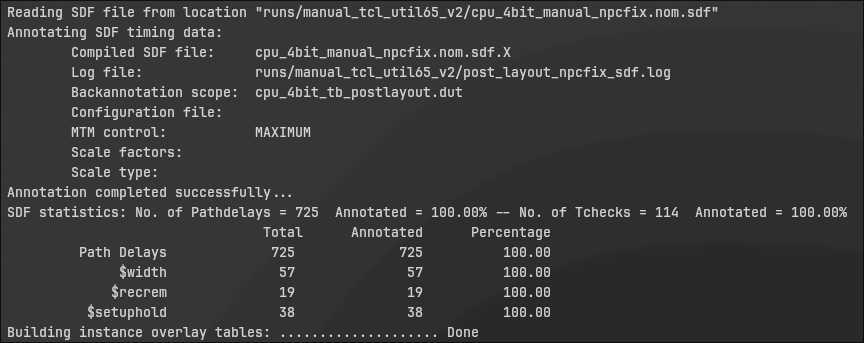
\includegraphics[width=0.86\textwidth,height=0.22\textheight,
    keepaspectratio]{22a.png}
  \caption*{(a) Kết quả SDF annotation}

  \vspace{0.4em}

  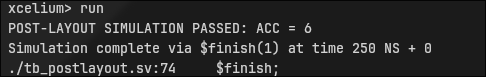
\includegraphics[width=0.60\textwidth,height=0.10\textheight,
    keepaspectratio]{22b.png}
  \caption*{(b) Kết quả testbench post-layout}

  \vspace{0.4em}

  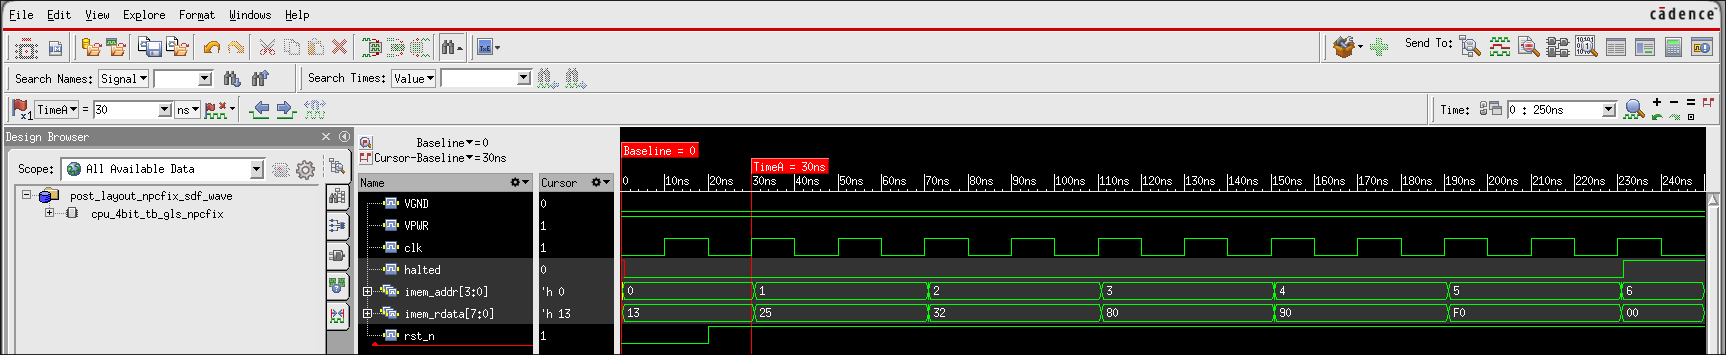
\includegraphics[width=0.96\textwidth,height=0.24\textheight,
    keepaspectratio]{22c.png}
  \caption*{(c) Waveform post-layout}
  \caption{Kết quả mô phỏng post-layout với SDF back-annotation.}
\end{figure}

\begin{figure}[H]
  \centering
  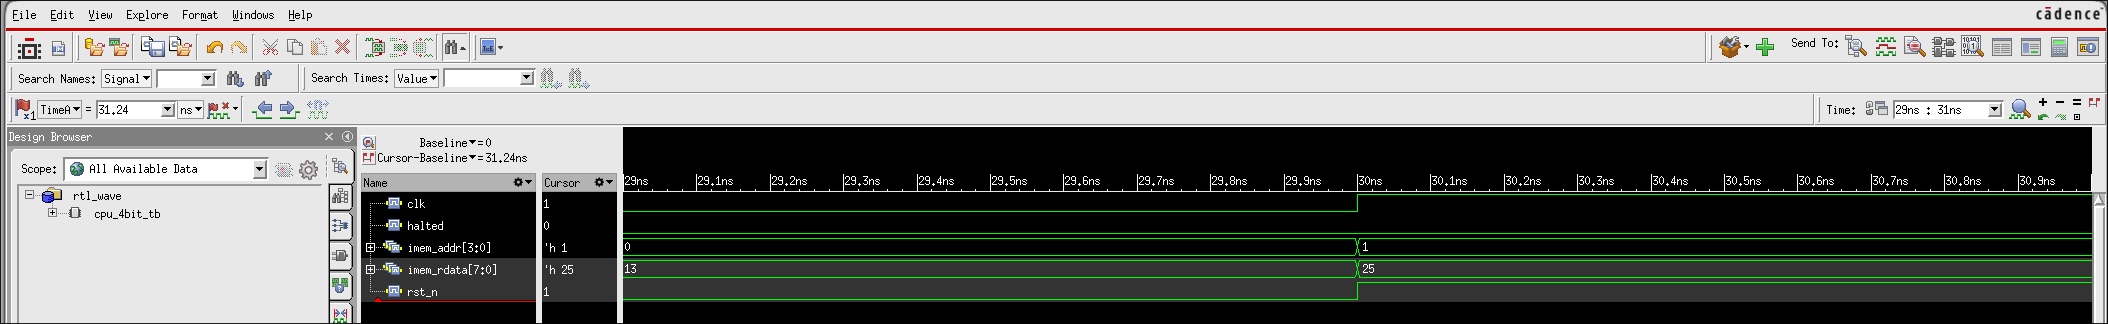
\includegraphics[width=0.96\textwidth,keepaspectratio]
    {23a.png}
  \caption*{(a) Waveform trước layout}

  \vspace{0.5em}

  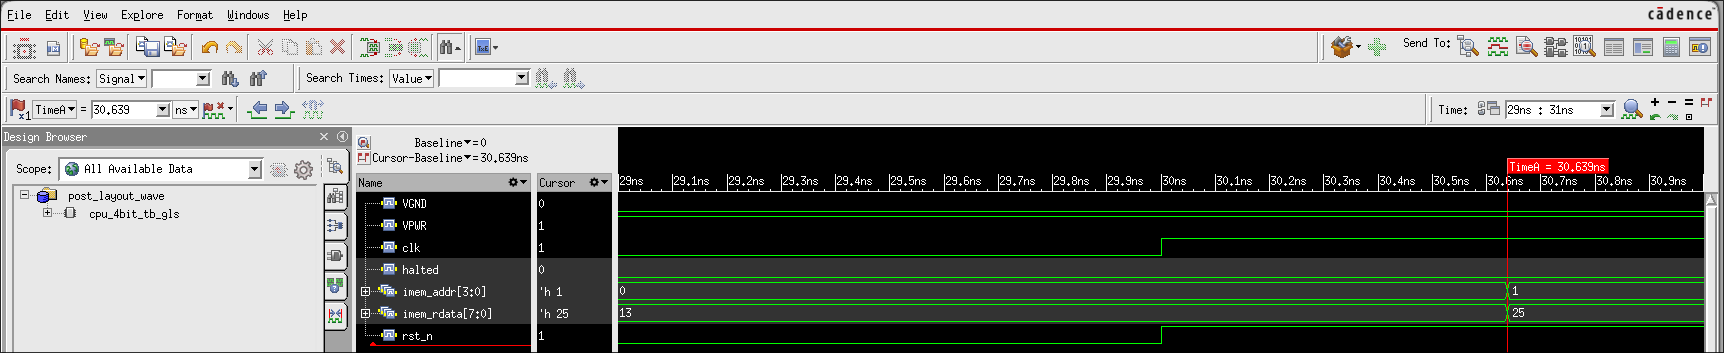
\includegraphics[width=0.96\textwidth,keepaspectratio]
    {23b.png}
  \caption*{(b) Waveform sau layout}
  \caption{So sánh waveform trước và sau layout; waveform sau layout thể
  hiện propagation delay sau SDF back-annotation.}
\end{figure}

\section{Tạo GDSII}

Sau khi hoàn tất trích xuất ký sinh, STA và mô phỏng post-layout, layout
cuối được stream-out thành file GDSII:

\begin{lstlisting}[language=tcl]
write_db cpu_4bit_manual_final.odb
write_def cpu_4bit_manual_final.def
global_connect
write_verilog -include_pwr_gnd cpu_4bit_manual_final.v
write_gds cpu_4bit_manual_final.gds
\end{lstlisting}

GDSII được mở trong KLayout để kiểm tra layout và thực hiện signoff DRC.

\reportfigure[0.88\textwidth]{24.png}
{Layout GDSII cuối được mở trong KLayout.}

\section{Kết quả DRC và LVS}

Kết quả signoff:

\begin{itemize}[noitemsep]
  \item KLayout DRC báo 0 violation;
  \item LVS báo layout và schematic match uniquely, với 153 device và
        159 net ở cả hai phía.
\end{itemize}

\reportpair{25a.png}
{KLayout DRC: 0 violation}
{25b.png}
{LVS: circuits match uniquely}
{Kết quả kiểm tra DRC và LVS.}

\section{Tổng hợp kết quả}

\begin{longtable}{>{\raggedright\arraybackslash}p{0.50\textwidth}
                  >{\raggedright\arraybackslash}p{0.32\textwidth}}
\toprule
\textbf{Chỉ tiêu} & \textbf{Kết quả} \\
\midrule
\endhead
Target core utilization & 65\% \\
Die area sau detailed routing & 4311.4448\umsq \\
Core area sau detailed routing & 2409.8112\umsq \\
Design area sau detailed routing & 1540\umsq \\
Utilization sau detailed routing & 64\% \\
Initial STA setup/hold slack & $+14.71/+0.27$\,ns \\
Sau repair setup/hold, TNS & $+14.70/+0.29$\,ns, 0 \\
Repair-design instances được thêm & 3 \\
CTS root/buffer/subnet/sink & 1/3/3/19 \\
Filler & Chỉ dùng \code{sky130_fd_sc_hd__fill*} \\
OpenROAD detailed-route DRC report & Rỗng \\
Antenna violations & 0 \\
Power-grid connectivity & VPWR/VGND connected \\
Post-route RCX setup slack & $+14.49$\,ns \\
Post-route RCX hold slack & $+0.26$\,ns \\
Post-route RCX TNS & $0.00$\,ns \\
KLayout signoff DRC & Pass: 0 violation \\
LVS & Match uniquely; 153 device, 159 net \\
SDF path-delay annotation & 722/722 \\
SDF timing-check annotation & 114/114 \\
RTL simulation & Pass, ACC = 6 \\
Post-layout simulation & Pass, ACC = 6 \\
\bottomrule
\end{longtable}

Các số liệu implementation và STA trong bảng thuộc flow physical design
được trình bày ở trên. Kết quả GLS được giữ lại từ lần mô phỏng
post-layout hiện có.

\section{Kết luận}

CPU 4-bit đã đi qua quy trình từ RTL đến artifact GDSII. Thiết kế RTL
được mô phỏng đúng, tổng hợp thành công sang standard cell Sky130, sau đó
trải qua floorplan, placement, CTS, routing, trích xuất ký sinh, STA và
mô phỏng post-layout. Thiết kế không có antenna violation, VPWR/VGND
được kết nối và đạt timing ở nominal corner với setup slack $+14.49$\,ns,
hold slack $+0.26$\,ns và TNS bằng 0 ở clock 20\,ns.

Mô phỏng post-layout có SDF tiếp tục cho kết quả ACC bằng 6 giống mô phỏng
RTL. Điều này xác nhận tính nhất quán chức năng của kết quả mô phỏng hiện
có. KLayout DRC báo 0 violation và LVS match uniquely với 153 device,
159 net.

\end{document}
